%% LaTeX example of poligraf.sty
\documentclass{article}
\usepackage[dvips]{color}
\usepackage[dvips]{graphicx}
\usepackage{poligraf}
%% --
\special{papersize=190mm,277mm}
%\special{papersize=180mm,267mm}
%% -- change some options ------
%\NoOverPrintBlack    % default overprint black
%\Separate\CYAN       % or
%\Separate\MAGENTA    % or
%\Separate\YELLOW     % or
%\Separate\BLACK   

%\xoffset{5}          % additional x an y offsets for printing on standard
%\yoffset{5}          % printer (do not use it for typesetters!)
%\cropmarkdistance{3} % 1--5 (default 3mm)
%\cropmarksize{10}    % default 10mm
%\barsize{6}          % default 6mm
%\nocolorbars         % no color bars and scales
%\onlycolorsteps      % color steps only
%\onlycolorbars       % color bars only
%\mirror              % mirror switch
%\labeloff            % no page label 

\begin{document}

\def\text{
\textcolor{red}{This is example of test page. This is example of test page.
This is example of test page. This is example of test page.
This is example of test page. This is example of test page.}\par
{\color{blue} This is example of test page. This is example of test page.
This is example of test page. This is example of test page.
This is example of test page. This is example of test page.}\par
\textcolor{green}{This is example of test page. This is example of test page.
This is example of test page. This is example of test page.
This is example of test page. This is example of test page.}\par
\textcolor{black}{This is example of test page. This is example of test page.
This is example of test page. This is example of test page.
This is example of test page. This is example of test page.}
}

% -----------------------------------------------------------
\text

\begin{figure}
 \begin{center}
  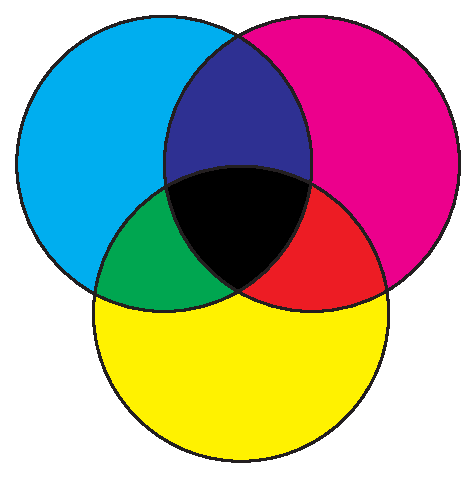
\includegraphics[width=0.5\hsize]{kol-cmyk}
  \caption{Vector graphics. CMYK model}
 \end{center}
\end{figure}

%% -----------------------------------------------------------
%%% put here your favourite colour photo 
%%% then uncomment the following lines and test colour separations
%\eject
%\begin{figure}
%\includegraphics[width=\hsize]{my-photo.eps}
%\caption{My photo}
%\end{figure}
% -----------------------------------------------------------

\end{document}
